\documentclass[compress]{beamer}
\usepackage{ifthen,verbatim}

\title{Alignment of the Muon System with HIP}
\author{Jim Pivarski, Alexei Safonov}
\institute{Texas A\&M University}
\date{29 June, 2007}

\newcommand{\isnote}{}
\xdefinecolor{lightyellow}{rgb}{1.,1.,0.25}
\xdefinecolor{darkblue}{rgb}{0.1,0.1,0.7}

%% %% Uncomment this to get annotations
%% \def\notes{\addtocounter{page}{-1}
%%            \renewcommand{\isnote}{*}
%% 	   \beamertemplateshadingbackground{lightyellow}{white}
%%            \begin{frame}
%%            \frametitle{Notes for the previous page (page \insertpagenumber)}
%%            \itemize}
%% \def\endnotes{\enditemize
%% 	      \end{frame}
%%               \beamertemplateshadingbackground{white}{white}
%%               \renewcommand{\isnote}{}}

%% Uncomment this to not get annotations
\def\notes{\comment}
\def\endnotes{\endcomment}

\setbeamertemplate{navigation symbols}{}
\setbeamertemplate{headline}{\includegraphics[height=1 cm]{../cmslogo} \hspace{0.1 cm} \includegraphics[height=1 cm]{../tamulogo} \hfill
\begin{minipage}{5.5 cm}
\vspace{-0.75 cm} \small
\begin{center}
\ifthenelse{\equal{\insertpagenumber}{1}}{}{\textcolor{blue}{\insertsection}}
\end{center}
\end{minipage} \hfill
\begin{minipage}{4.5 cm}
\vspace{-0.75 cm} \small
\begin{flushright}
\ifthenelse{\equal{\insertpagenumber}{1}}{}{Jim Pivarski \hspace{0.5 cm} \insertpagenumber\isnote/\pageref{numpages}}
\end{flushright}
\end{minipage}\mbox{\hspace{0.2 cm}}}

\begin{document}
\frame{\titlepage}

\begin{notes}
\item This is the annotated version of my talk.
\item If you want the version that I am presenting, download the one
labeled ``slides'' on Indico (or just ignore these yellow pages).
\item The annotated version is provided for extra detail and a written
record of comments that I intend to make orally.
\item Yellow notes refer to the content on the {\it previous} page.
\item All other slides are identical for the two versions.
\end{notes}

\begin{frame}
\frametitle{Introduction: monitoring tools (we'll be using it later\ldots)}
\begin{enumerate}
\item CommonAlignmentMonitor: general plotting package integrated into AlignmentProducer
\begin{itemize}
\item Manages iteration, collection after parallel processing
\end{itemize}
\item \textcolor{blue}{AlignmentMonitorMuonHIP outputs histograms for every chamber (or every layer): residuals versus everything}
\item \textcolor{blue}{pyROOT script merges histograms on the fly}
\end{enumerate}
\begin{center}
\includegraphics[width=0.8\linewidth]{realplots/monitoring_tool}

\textcolor{blue}{all of this will be in CVS early next week}
\end{center}
\end{frame}

\begin{notes}
\small
\item Command for the featured plot: ``r.select(lambda c, h: not c.barrel and h.GetEntries() $>$ 0)''
\item Can pass arbitrary Python functions to select by chamber information (c) or histogram features (h)
\item Almost as much versatility as an ntuple, this tool will allow us to
``zoom in'' on alignment problems, to understand specific outliers and
allow human decision-making in early data
\item ROOT file sizes are $\sim$10 MB per iteration
\item A link to information about Javier's analyzer: http://indico.cern.ch/conferenceDisplay.py?confId=13742
\item Due to the way we do track refitting, the integrated monitor is
sensitive to updated residuals but not updated track parameters.
Thus, we can use AlignmentMonitorMuonHIP to see narrowing
residuals/$\chi^2$, and then re-reconstruct from scratch with Javier's
analyzer to see the change in $p_T$ distributions, the $Z'$ peak,
Drell-Yan seepage, etc.
\end{notes}

\begin{frame}
\frametitle{Muon alignment simulation}
\begin{itemize}\setlength{\itemsep}{0.25 cm}
\item First full-scale muon alignment in AlignmentProducer

\begin{itemize}\setlength{\itemsep}{0.25 cm}
\item Large dataset: 10 pb$^{-1}$ of muons from $W$ and $Z$ (simulated by $Z$ only)
\item Full precision goals (200 $\mu$m)
\item Random misalignments with SurveyOnlyScenario (rather than moving all chambers in the same direction)
\end{itemize}

\item Two major approaches, developed simultaneously

\begin{itemize}\setlength{\itemsep}{0.25 cm}
\item Align the muon system to the tracker (globalMuons)
\begin{itemize}
\item converges more quickly
\end{itemize}

\item Align the muon system to itself (standAloneMuons)
\begin{itemize}
\item independent of the tracker
\end{itemize}
\end{itemize}
\end{itemize}
\end{frame}

\begin{frame}
\frametitle{Aligning to the tracker}
\begin{itemize}
\item Residuals from globalMuons have two peaks per chamber, due to track-fitting bias
\end{itemize}

\begin{tabular}{p{0.4\linewidth} p{0.6\linewidth}}
\begin{minipage}{\linewidth}
\includegraphics[width=3 cm, angle=90]{realplots/bias_residual_globalMuon}
\end{minipage} &
\begin{minipage}{\linewidth}
\begin{center}
\includegraphics[height=3 cm]{realplots/two_cases.pdf}
\end{center}
\end{minipage} \\
 & \\
\begin{minipage}{\linewidth}
\includegraphics[width=3 cm, angle=90]{realplots/bias_residual_tracker-to-muon}
\end{minipage} &
\begin{minipage}{\linewidth}
\begin{itemize}
\item Simply extrapolating a tracker track into the muon system removes the bias, but at a severe resolution cost (note wider scale)
\item Neither is optimal
\end{itemize}
\end{minipage}
\end{tabular}
\end{frame}

\begin{notes}
\item The tracker-to-muon extrapolation is what I presented in my last EMU talk at UCLA
\item Alignment resolution was $\sim$4 mm
\end{notes}

\begin{frame}
\frametitle{The ``lowbias'' method}
\begin{itemize}
\item Re-fit globalMuon tracks with inflated hit uncertainties in the muon system
\item Resulting tracks are determined mostly by the silicon tracker, but they ``know'' about scattering in the muon system
\end{itemize}
\begin{center}
\includegraphics[height=0.7\linewidth, angle=90]{realplots/bias_residual_lowbias}
\end{center}
\end{frame}

\begin{notes}
\item The tall peak at 1 cm is the misalignment, small peak at 0 is due to bias
\item Usually converges in one iteration
\end{notes}

\begin{frame}
\frametitle{The ``standalone'' method}
\begin{itemize}
\item standAloneMuons have the two-peak structure in residuals, and therefore need to iterate to decouple track-fitting from chamber alignment
\item With a $|\mbox{residuals}| <$ 5 cm cut, this method shows clear convergence for most chambers:
\begin{center}
\includegraphics[height=0.48\linewidth, angle=90]{realplots/standalone_converges}
\includegraphics[height=0.48\linewidth, angle=90]{realplots/standalone_residuals}
\end{center}

\item We are keenly interested in saving the tails\ldots
\end{itemize}
\end{frame}

\begin{notes}
\item We need to study the outliers!  Figure out what's happening to
the tails!  Find a way to diagnose it in data, also (shape of residual
distribution?)

\item Muon alignment is especially important for keeping Drell-Yan
backgrounds from smearing into high dimuon-mass channels for New
Physics.  We therefore care very much about the higher moments of the
$p_T$ distribution, which is to say, alignment outliers.
\end{notes}

\begin{frame}
\frametitle{The same plots for ``lowbias''}
\begin{center}
\includegraphics[height=0.48\linewidth, angle=90]{realplots/lowbias_converges}
\includegraphics[height=0.48\linewidth, angle=90]{realplots/lowbias_residuals}
\end{center}
\begin{itemize}
\item Converges in one iteration
\item Beyond that most chambers are stable, but a few DTs wander
\item There's also a cumulative problem with hit efficiency
\end{itemize}
\end{frame}

\begin{frame}
\frametitle{Alignment Results (10 pb$^{-1}$)}
\begin{itemize}\setlength{\itemsep}{0.25 cm}
\item Starting from MuonSurveyOnlyScenario: positions misaligned 2.5 mm, $\phi_z$ misaligned 0.25 mrad

\item Five degrees of freedom in alignment: $x$, $y$, $\phi_x$, $\phi_y$, $\phi_z$

\item Accuracy: \textcolor{blue}{one iteration lowbias}, \textcolor{red}{ten iterations standalone}
\begin{center}
\begin{tabular}{c c}
\includegraphics[height=0.4\linewidth, angle=90]{realplots/x_positions} &
\includegraphics[height=0.4\linewidth, angle=90]{realplots/y_positions} \\
$x_{\mbox{\scriptsize aligned}} - x_{\mbox{\scriptsize true}}$ (cm) &
$y_{\mbox{\scriptsize aligned}} - y_{\mbox{\scriptsize true}}$ (cm)
\end{tabular}
\end{center}

\item Precision: alignment uncertainties are underestimated by a factor of 3--4 (pull distribution is wide)
\end{itemize}
\end{frame}

\begin{frame}
\frametitle{Figures of merit}
\vspace{-0.75 cm}
\begin{columns}
\column{0.4\linewidth}
\begin{enumerate}
\item $\sigma$ of core Gaussian (best-measured chambers)
\item RMS, cut at 1 cm
\item $|\mbox{max}|$ (worst outlier)
\end{enumerate}

\column{0.6\linewidth}
\begin{center}
\begin{tabular}{c | c c c}
790 chambers & core $\sigma$ & RMS & $|\mbox{max}|$ \\\hline
\textcolor{blue}{lowbias $x$} & \textcolor{blue}{50} & \textcolor{blue}{280} & \textcolor{blue}{4500} \\
\textcolor{blue}{lowbias $y$} & \textcolor{blue}{270} & \textcolor{blue}{860} & \textcolor{blue}{6000} \\
\textcolor{red}{standalone $x$} & \textcolor{red}{50} & \textcolor{red}{1040} & \textcolor{red}{$\infty$} \\
\textcolor{red}{standalone $y$} & \textcolor{red}{290} & \textcolor{red}{1540} & \textcolor{red}{34000} \\
\end{tabular}
\mbox{ } \hfill microns
\end{center}

\end{columns}

\vfill
\includegraphics[height=0.48\linewidth, angle=90]{realplots/lowbias_fit}
\includegraphics[height=0.48\linewidth, angle=90]{realplots/standalone_fit} \\
\end{frame}

\begin{notes}
\small
\item Fits are purely Gaussian on a restricted range: $\pm$100 $\mu$m for $x$ and $\pm$500 $\mu$m for $y$.
\item The RMS that I quote is cut at 1 cm (as stated on the previous page).  The RMS that ROOT reports in its statistics boxes is cut to the current window width, and I zoom into some of the plots for detail.  Therefore, ROOT sometimes a different RMS in its statistics box than I quote in the table and in plots on the next few pages.  I was careful to always use a 1 cm cut in all the numbers I report!
\item $|\mbox{max}|$ is extremely twitchy, as you may imagine.  These $|\mbox{max}|$ numbers are dominated by the few chambers that diverge, so the numerical value doesn't have a precise meaning, it's only a guide to say that I still have divergent chambers.  It will become more useful when I fix that DT problem.
\item For the sake of the table, I selected the largest ``reasonable'' value.  A few values were 5098450298475e+4598; I skipped those.  In the case labelled with an $\infty$, there wasn't a clear break between reasonable and unreasonable.
\end{notes}

\begin{frame}
\frametitle{Figures of merit versus iteration}
\begin{columns}
\column{0.48\linewidth}
\begin{center}
\includegraphics[width=\linewidth]{realplots/x_width_vsiter_lowbias}
\end{center}
\column{0.48\linewidth}
\begin{center}
\includegraphics[width=\linewidth]{realplots/x_width_vsiter_standalone}
\end{center}
\end{columns}
\begin{itemize}
\item Core $\sigma$ largely unchanged after first iteration
\item standalone method requires 7 iterations
\end{itemize}
\end{frame}

\begin{frame}
\frametitle{Figures of merit versus integrated luminosity}
\begin{columns}
\column{0.48\linewidth}
\begin{center}
\includegraphics[width=\linewidth]{realplots/lowbias_width_vsevents}
\end{center}
\column{0.48\linewidth}
\begin{center}
\includegraphics[width=\linewidth]{realplots/standalone_width_vsevents}
\end{center}
\end{columns}
\begin{itemize}
\item lowbias reaches sensitivity limit between 10 and 100 pb$^{-1}$
\item standalone technique reaches limit below 10 pb$^{-1}$
\end{itemize}
\end{frame}

\begin{notes}
\item That second plot looks very strange because the high-luminosity
point actually has less resolution than the low luminosity point.  If
you look at the corresponding resolution vs.\ iteration, you'll see
that this difference is in the noise.  If I assigned errorbars, the
points would be consistent.

\includegraphics[width=0.5\linewidth]{realplots/x_width_vsiter_standalone_100}
\end{notes}

\begin{frame}
\frametitle{{\it Initial} diagnostics of the outliers}
\begin{itemize}
\item Just apply the tool to the chambers that diverge
\item $x$ beyond 0.8 cm in the second iteration (standalone):
\end{itemize}

\vfill
\begin{columns}
\column{0.35\linewidth}
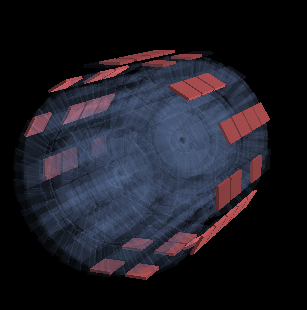
\includegraphics[width=\linewidth]{divergent_chambers.png}
\column{0.5\linewidth}
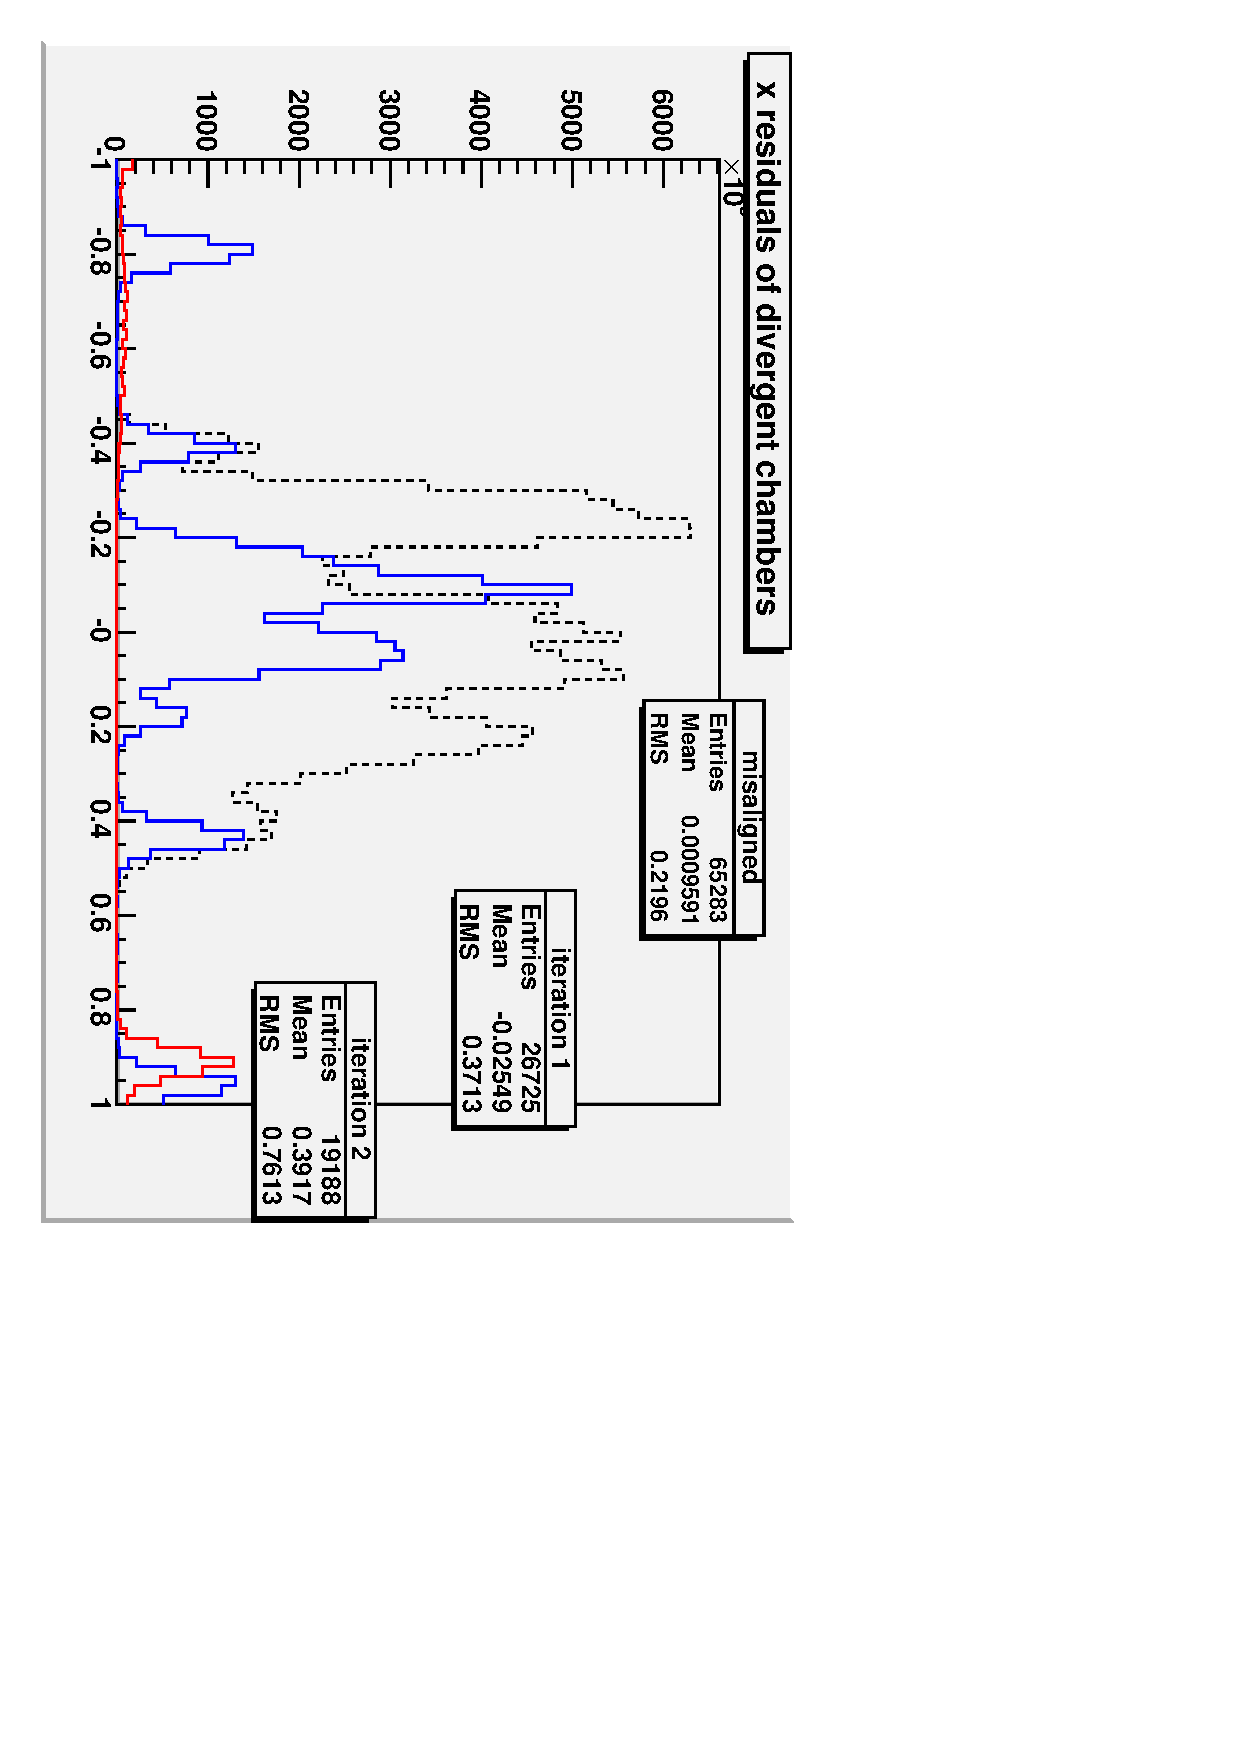
\includegraphics[height=1.2\linewidth, angle=90]{divergent_chambers.pdf}
\end{columns}
\end{frame}

\begin{frame}
\frametitle{The imperfectly-aligned chambers}
\begin{itemize}
\item $x$ between 0.02 and 0.1 cm in the tenth iteration (standalone):
\end{itemize}

\vfill
\begin{columns}
\column{0.35\linewidth}
\only<1>{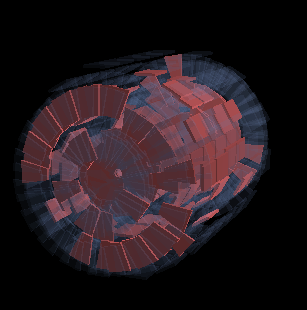
\includegraphics[width=\linewidth]{inthetails1.png}}
\only<2>{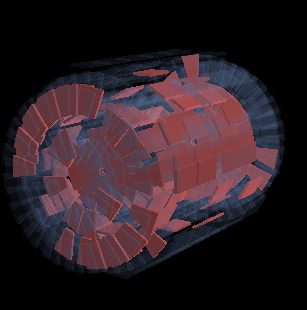
\includegraphics[width=\linewidth]{inthetails2.png}}
\only<3>{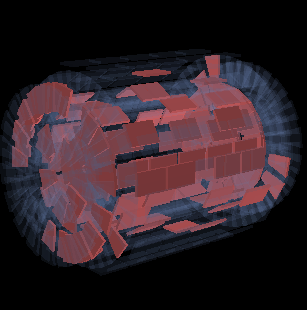
\includegraphics[width=\linewidth]{inthetails3.png}}
\only<4>{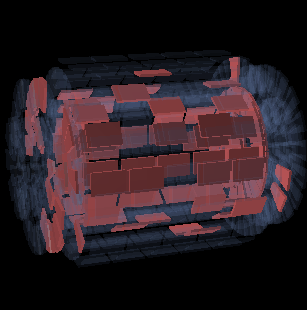
\includegraphics[width=\linewidth]{inthetails4.png}}
\only<5>{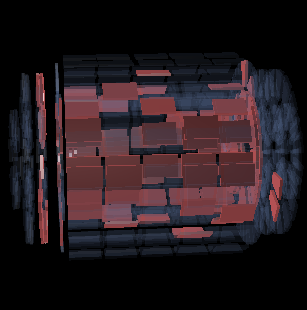
\includegraphics[width=\linewidth]{inthetails5.png}}
\column{0.5\linewidth}
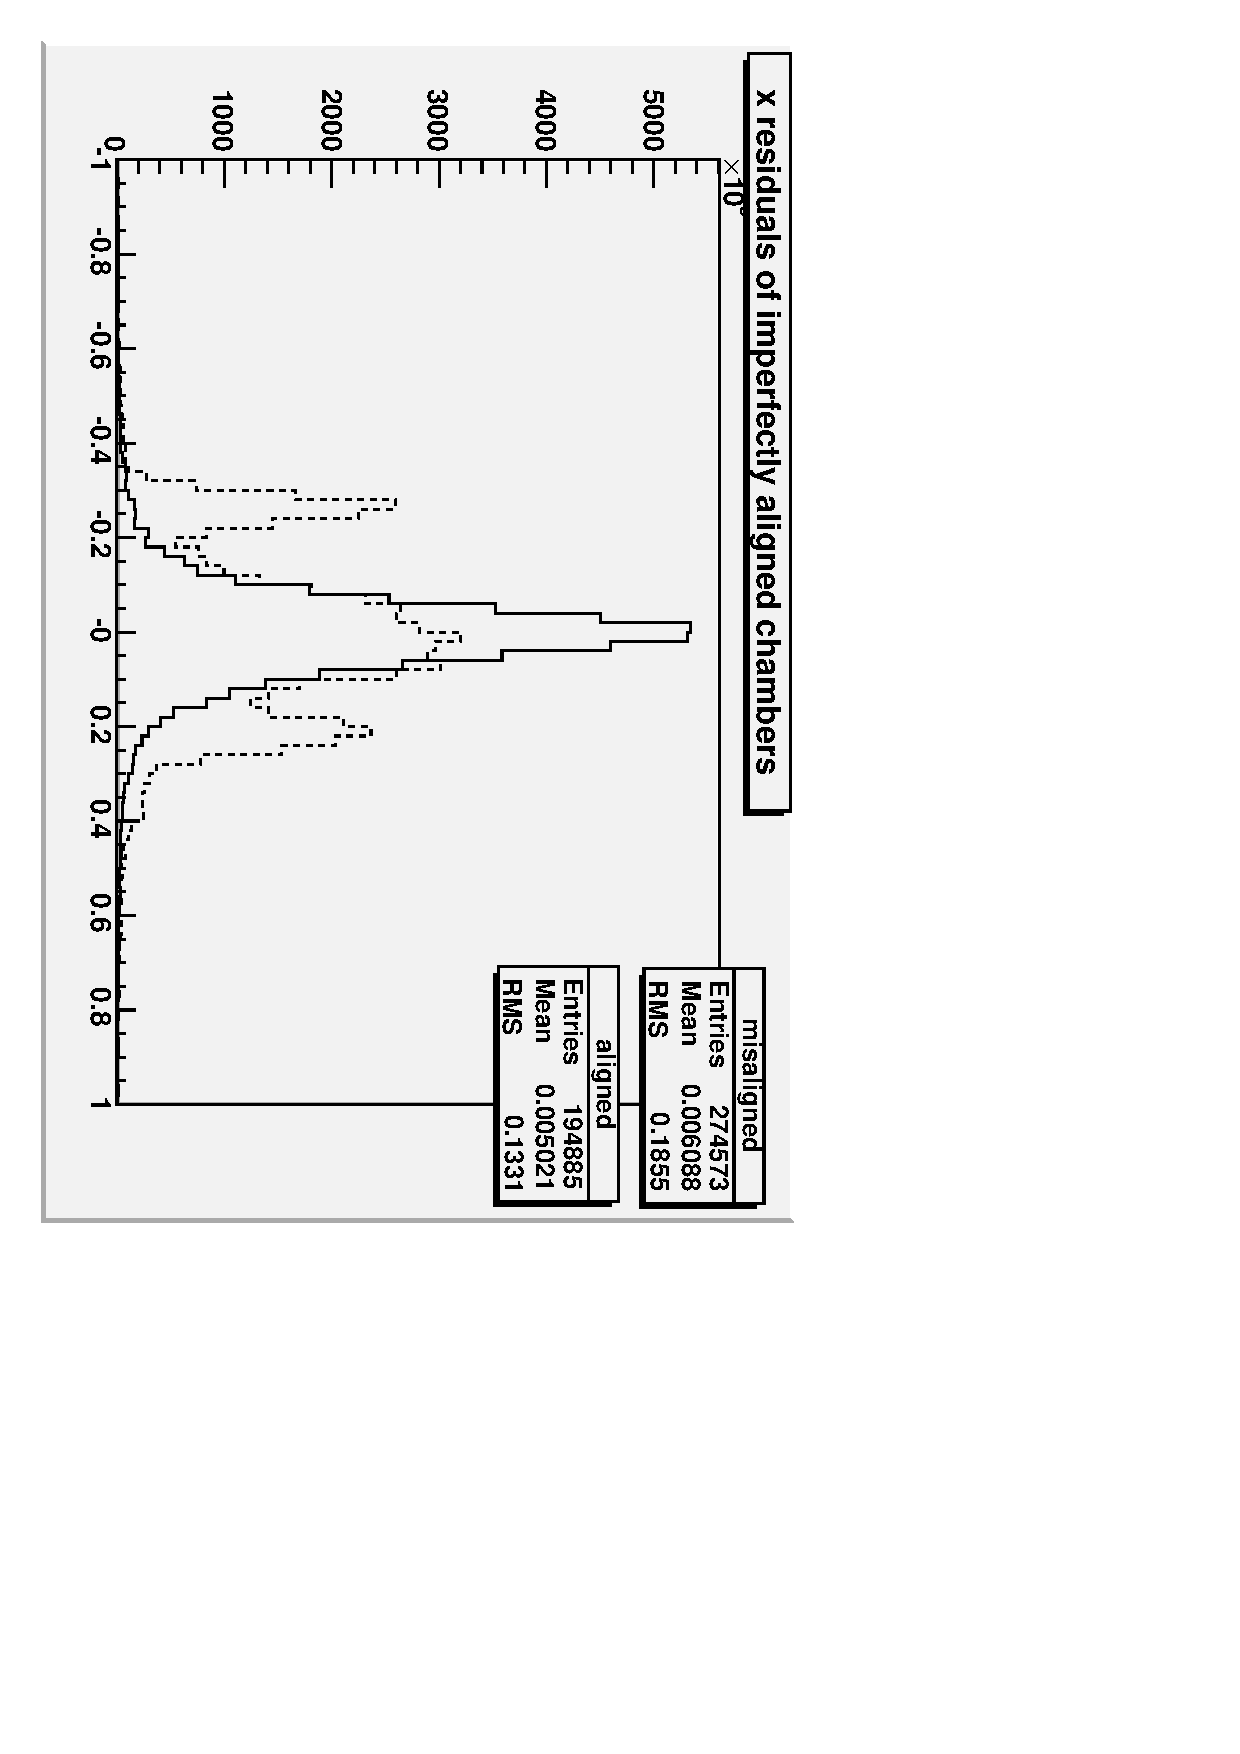
\includegraphics[height=1.2\linewidth, angle=90]{inthetails.pdf}
\end{columns}
\end{frame}

%% \begin{frame}
%% \frametitle{Context: Karoly Banicz's (re-)discovery of layer offsets}
%% \begin{columns}
%% \column{0.3\linewidth}
%% \begin{itemize}
%% \item Agrees with production site measurements
%% \item \textcolor{blue}{We want to reproduce this study in AlignmentProducer}
%% \end{itemize}
%% \column{0.7\linewidth}
%% \includegraphics[width=\linewidth]{realplots/karolys_layers}
%% \end{columns}

%% \begin{center}
%% \begin{tabular}{c | c c c}
%% 120 aligned layer positions & mean & stdev & $|\mbox{max}|$ \\ \hline
%% $x$ & -55 $\mu$m & 190 $\mu$m & 670 $\mu$m \\
%% $y$ & 110 $\mu$m & 330 $\mu$m & 1.2 mm \\
%% $\phi_z$ & 0.01 mrad & 0.04 mrad & 0.15 mrad
%% \end{tabular}
%% \end{center}
%% \end{frame}

%% \begin{frame}
%% \frametitle{Preliminary MTCC alignment with AlignmentProducer}
%% \begin{itemize}\setlength{\itemsep}{0.25 cm}
%% \item Alignment attempts were beset by random crashes
%% \item A single standalone iteration survived; not enough for a reliable alignment, but enough for order-of-magnitude

%% \vspace{0.25 cm}
%% \begin{center}
%% \begin{tabular}{c | c c c}
%% 102 semi-aligned layer positions & mean & stdev & $|\mbox{max}|$ \\ \hline
%% $x$ & 8 $\mu$m & \textcolor{blue}{192 $\mu$m} & 440 $\mu$m
%% \end{tabular}
%% \end{center}

%% \vspace{0.25 cm}
%% \item in rough agreement with Karoly's results

%% \vfill
%% \item We'll need more data and more robust computation
%% \item Likely to get both with MTCC 1\_5\_0 re-reconstruction
%% \end{itemize}
%% \end{frame}

\begin{frame}
\frametitle{Aligning individual layers}
\begin{itemize}
\item CSC chambers known to have 100-300 $\mu$m offsets (MTCC)
\item The near-tails are bigger (this is 100 pb$^{-1}$, $x$, $y$, $\phi_z$ only)
\end{itemize}

\includegraphics[height=0.48\linewidth, angle=90]{realplots/layer_x_lowbias_fit}
\includegraphics[height=0.48\linewidth, angle=90]{realplots/layer_x_standalone_fit}

\vfill
\begin{center}
\mbox{\begin{minipage}{0.6\linewidth}
\begin{tabular}{c | c c c}
3920 layers & core $\sigma$ & RMS & $|\mbox{max}|$ \\\hline
\textcolor{blue}{lowbias $x$} & \textcolor{blue}{50} & \textcolor{blue}{1630} & \textcolor{blue}{6600} \\
\textcolor{blue}{lowbias $y$} & \textcolor{blue}{360} & \textcolor{blue}{1830} & \textcolor{blue}{13000} \\
\textcolor{red}{standalone $x$} & \textcolor{red}{60} & \textcolor{red}{1720} & \textcolor{red}{6600} \\
\textcolor{red}{standalone $y$} & \textcolor{red}{380} & \textcolor{red}{1970} & \textcolor{red}{6400} \\
\end{tabular}
\mbox{ } \hfill microns
\end{minipage}}
\end{center}
\end{frame}

\begin{frame}
\begin{center}
\includegraphics[height=0.48\linewidth, angle=90]{realplots/layer_x_width_vsiter_standalone.pdf}

\includegraphics[height=0.48\linewidth, angle=90]{realplots/layer_lowbias_width_vsevents.pdf}
\includegraphics[height=0.48\linewidth, angle=90]{realplots/layer_standalone_width_vsevents.pdf}
\end{center}
\end{frame}

\begin{frame}
\frametitle{Whole-disk/wheel alignment is also important}
\begin{itemize}
\item 0.7 cm disk misalignment observed in MTCC phase 2
\item How many tracks does HIP need?
\item Not many: $x$,$y$ to 800 $\mu$m with 300 tracks
\end{itemize}
\begin{center}
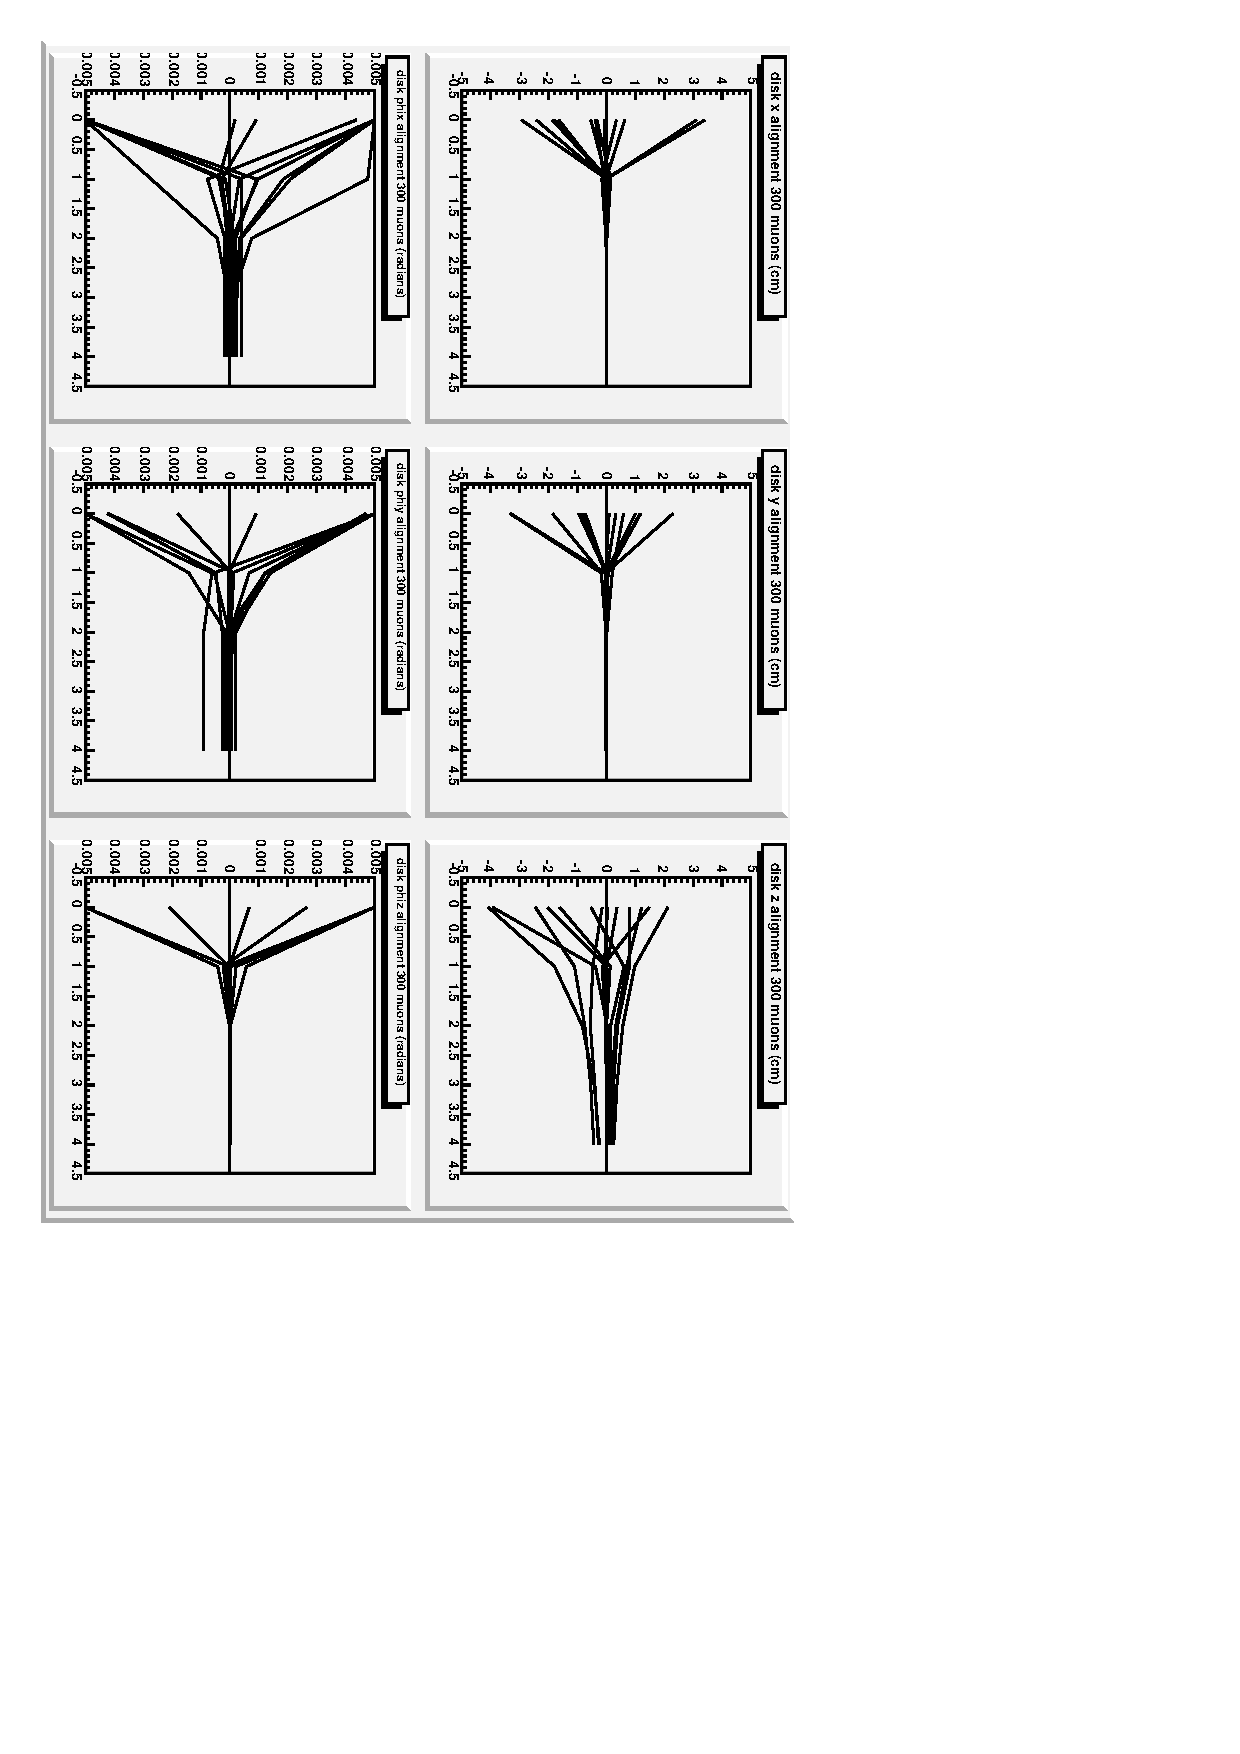
\includegraphics[height=0.7\linewidth, angle=90]{convergence_g300.pdf}
\end{center}
\mbox{ } \hfill \small top row: $x$, $y$, $z$ (cm), bottom: $\phi_x$, $\phi_y$, $\phi_z$ (rad)
\end{frame}

\begin{frame}
\frametitle{Summary}
\begin{itemize}\setlength{\itemsep}{0.25 cm}
\item Overall scheme and infrastructure components are now mature
\item Entering the era of precision alignment studies
\item Procedure is ready for CSA07, some updates need to be checked into CVS
\item We have taken a first glance at MTCC data and are ready to apply our software to 1\_5\_0 re-reconstructed data
\item Concrete list of systematics studies planned for CSA07
\item The software is available for cosmic ray/beam halo studies\ldots
\item We're starting to write a CMS Note
\end{itemize}
\label{numpages}
\end{frame}

\end{document}
